\subsection{Membership Implementation}

As covered in Section \ref{sssec:member}, the Membership trapezia would be defined within the system, rather than dynamically being calculated. This made use of the Fuzzy Logic Toolbox by leveraging the following functions:

\begin{itemize}
  \item \textbf{trapmf: } trapezium-shaped membership function
  \item \textbf{evalmf: } a generic membership evaluation function
\end{itemize}

Having pre-defined functions for creating and evaluating the membership trapezia ensured that the function was a quick implementation. However it did reduce the number of Unit Tests I could have written to test the creation of such elements.

In this function, an image is read in, the membership of each pixel is evaluated against each of the two or three membership trapezia, adding the outcome to a corresponding array (e.g. one array for the membership of all the pixels against the low-trapezium etc). The two/three arrays (depending on number of trapezia) are then compared and the array which has the greater membership for each pixel, that membership value is added to another array which compiles all the highest values.

For example:

\begin{minted}
  [
  breaklines,
  frame=lines,
  framesep=2mm,
  baselinestretch=1.2,
  fontsize=\small,
  linenos
  ]
  {text}
    pixel[1,1]`s membership in trapezium low = 0.8
    pixel[1,1]`s membership in trapezium medium = 0.4
    pixel[1,1]`s membership in trapezium high = 0

    Therefore as 0.8 is the highest membership value, this is added to the image membership array
\end{minted}

The three/four arrays (one for each trapezium and one for the highest values) are then passed out of the function, and utilised in each of the algorithm functions.

\subsection{GUI Implementation}

Initially the \acrfull{GUI} would be implemented using JavaFX, and any MATLAB additions would be linked in, however it`s possible to create \acrshort{GUI}s easily within MATLAB itself. GUIDE \cite{guide} is MATLAB`s Application development environment where you can either build using purely drag-and-drop techniques, program the application as standard in the editor, or both.

The combination of both the drag-and-drop environment, and manually programming via the editor was undertaken during this project, to allow a greater amount of freedom and flexibility. Drag-and-drop was leveraged to style the \acrshort{GUI} and the editor was used to program the functionality in the back-end and link in the \Gls{Congealing} and Fuzzy Entropy algorithms.

\vspace{1cm}
\subsection{Algorithm Implementation}

Details of the implementation of the Fuzzy Entropy Algorithms can be found:

\textbf{Shannon Entropy: } Subsection \ref{ssec:shannon-entropy}

\textbf{Non-Probabilistic Entropy: } Subsection \ref{ssec:non-prob-sec}

\textbf{Hybrid Entropy: } Subsection \ref{ssec:hybrid-sec}

\subsection{Data Flow}

\begin{figure}[H]
  \centering
  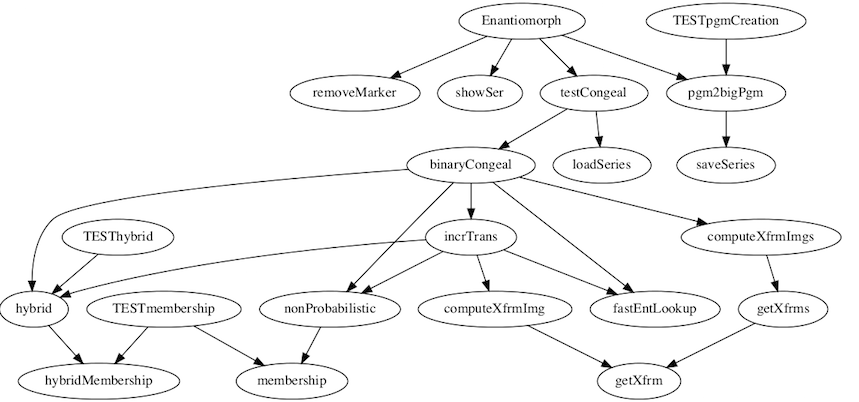
\includegraphics[width=\textwidth]{Chapter2/software-img/data_flow_2.png}
  \caption{Data flow through the application.}
  \label{fig:data-flow}
\end{figure}

Figure \ref{fig:data-flow} shows the flow of data through the application, all the way up to \texttt{Enantiomorph} the \acrshort{GUI}. This diagram shows the integration of new, modified and existing functions/scripts in the code-base, as listed in Appendix \ref{appendix:code}

\subsection{Testing}

Prior to the project beginning, it was outlined that this project should follow a \acrshort{TDD} practice. In \acrshort{TDD}, the Developer first writes a test, which will fail due to the lack of corresponding functionality. They would then go on to implement the functionality desired by the test. Finally, any refactoring of the initial test and/or code would take place.

However due to the nature of the research, it became increasingly more difficult to follow given the research which had to be undertaken alongside development. This led to a change from \acrshort{TDD} to Retrospective Testing, in which I would write all tests, post functional implementation. This is a more traditional approach to testing, and still catches the same errors which might occur during \acrshort{TDD}.

\subsubsection{Unit Tests}

Unit Tests were completed using MATLAB`s Unit Testing Framework \cite{testing}, which covers all the ways in which you can program in MATLAB:

\begin{itemize}
  \item Script-Based Unit Tests
  \item Function-Based Unit Tests
  \item Class-Based Unit Tests
  \end{itemize}

The majority of my work in MATLAB was Function-based, so this was the style followed for unit tests.

\begin{figure}[H]
  \centering
  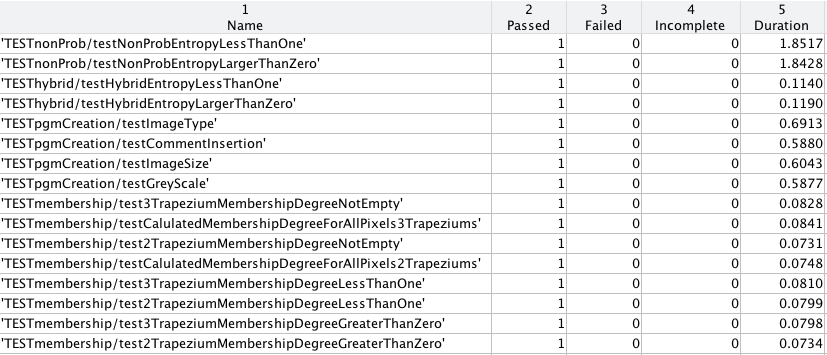
\includegraphics[width=\textwidth]{Chapter2/software-img/test-results.png}
  \caption{Results from MATLAB Unit Tests.}
  \label{fig:unit-test-results}
\end{figure}

As Figure \ref{fig:unit-test-results} demonstrates, all Unit tests passed.

\subsubsection{Acceptance Tests}

Table \ref{table:acceptance} outlines the results from the Acceptance Tests run. The left-most column \say{User Story Reference} aligns with Table \ref{table:User Stories}, so more detail can be found.

\begin{center}
  \small
  \begin{longtable}{| p{3cm} | p{4cm} | p{4cm}  | p{3cm} | p{2cm} |}
    \hline
      \textbf{User Story Reference} & \textbf{Expected Outcome} & \textbf{Actual Outcome} & \textbf{Pass/Fail} \\
      1 & Image is loaded into the system & As expected & Pass \\ \hline
      2 & Membership array is passed out of the membership function and is usable in other functions & As expected & Pass \\ \hline
      3 & Images are aligned using Non-Probabilistic entropy and the output \& entropy outputs are realistic & As expected & Pass \\ \hline
      4 & Images are aligned using the metric the user has selected when running the function & As expected & Pass \\ \hline
      6 & The number of iterations is run as specified by the User, then function stops & As expected & Pass \\ \hline
      8 & Images are aligned using Shannon entropy and the output \& entropy outputs are realistic & As expected & Pass \\ \hline
      9 & Image(s) selected to be loaded into the GUI is displayed & As expected & Pass \\ \hline
      12 & Image box where input image appears goes blank after Clear button is selected & As expected & Pass \\ \hline
      13 & Images are aligned using Hybrid entropy and the output \& entropy outputs are realistic & As expected & Pass \\ \hline
      14 & Images are aligned using the chosen alignment metric & As expected & Pass \\ \hline
      15 & The number of iterations is run as specified by the User, then function stops & As expected & Pass \\ \hline
      16 & When an input image is loaded in, Metadata is displayed in the GUI about the image & As expected & Pass \\ \hline
      17 & After \Gls{Congealing}, the user can press the \say{See all Mean images} button and a new Figure displays the mean image after each iteration & As expected & Pass \\ \hline
      18 & After \Gls{Congealing}, the user can press the \say{See Adjusted Inputs} button and a new Figure displays the adjusted input images after the final iteration  & As expected & Pass \\ \hline
      21 & Image box where output image appears goes blank after Clear button is selected along with all other fields & As expected & Pass \\ \hline
      22 & Image is displayed larger in a new Figure & As expected & Pass \\ \hline
      23 & Save file dialog appears with a sensible name suggested (i.e. final image - alignment-chosen - number of iterations) & As expected & Pass \\ \hline
      24 & When \say{Entropy details} button is selected, a new Figure appears with a graph showing entropy decrease. Final Entropy \& time taken also displays in the main GUI & As expected & Pass \\ \hline
      25 & Egg-timer appears when \Gls{Congealing} Algorithm is running & As expected & Pass \\ \hline
      \caption{Acceptance Test results}
      \label{table:acceptance}
  \end{longtable}
\end{center}
